% !TEX TS-program = pdflatex
% !TEX encoding = UTF-8 Unicode
\documentclass[12pt]{article} 

\usepackage[utf8]{inputenc} 
\usepackage{geometry} 
\geometry{a4paper} 
\geometry{margin=0.25in} 
\geometry{portrait} 

\usepackage{tikz} 

\usepackage{amsmath} 
\usepackage{physics} 
\title{once more tikz}
\author{vijayabhaskar badireddi} 

\usetikzlibrary{through,intersections}

\begin{document}

\section*{Solution}

\begin{center}
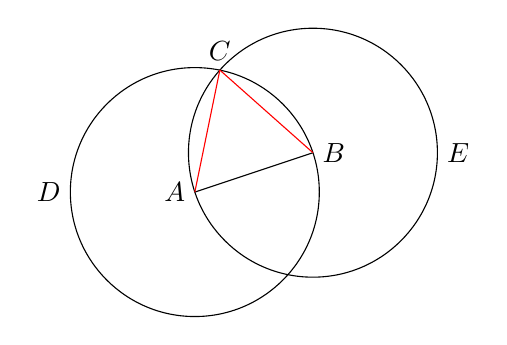
\begin{tikzpicture}
\coordinate [label=left:$A$] (A) at (0,0);
\coordinate [label=right:$B$] (B) at (1.5,0.5);
\draw (A) -- (B);
\node [name path=D,draw,circle through=(B),label=left:$D$] at (A) {};
\node [name path=E,draw,circle through=(A),label=right:$E$] at (B) {};

\path [name intersections={of=D and E}];
\coordinate [label=above:$C$] (C) at (intersection-1);
\draw [red] (A) -- (C);
\draw [red] (B) -- (C);

\end{tikzpicture}
\end{center}

\end{document}
